\documentclass{beamer}
\usepackage[latin1]{inputenc}
\usepackage{times}
\usepackage{tikz}
\usetheme{Luebeck}
%\usecolortheme{albatross}
\usepackage{amsmath,amsfonts,amsthm,amssymb}
\usepackage{setspace}
\usepackage{Tabbing}
\usepackage{fancyhdr}
\usepackage{lastpage}
\usepackage{extramarks}
\usepackage{chngpage}
\usepackage{soul,color}
\usepackage{graphicx,float,wrapfig}
\usepackage{xcolor}
\usepackage{listings}
\usepackage{float}
%\usepackage{subfloat}
\usepackage{subfigure}
\usepackage{caption}
\usepackage{enumitem}
\usepackage{algpseudocode}

\definecolor{darkorange}{RGB}{240, 120, 0}
\definecolor{darkgreen}{RGB}{0, 128, 0}
\definecolor{darkred}{RGB}{128, 0, 0}

\setbeamercolor{background canvas}{bg=white}
\setbeamercolor{frametitle}{fg=white, bg=darkorange}
\setbeamercolor{normal text}{bg=black,fg=black}
\setbeamercolor{structure}{bg=black, fg=darkorange}


\lstdefinestyle{customc}{
  belowcaptionskip=1\baselineskip,
  breaklines=true,
  frame=L,
  xleftmargin=\parindent,
  language=Python,
  showstringspaces=false,
  basicstyle=\footnotesize\ttfamily,
  keywordstyle=\bfseries\color{green!40!black},
  commentstyle=\itshape\color{purple!40!black},
  identifierstyle=\color{blue},
  stringstyle=\color{orange},
}

\lstdefinestyle{customc}{
  belowcaptionskip=1\baselineskip,
  breaklines=true,
  frame=L,
  xleftmargin=\parindent,
  language=Python,
  showstringspaces=false,
  basicstyle=\footnotesize\ttfamily,
  keywordstyle=\bfseries\color{green!40!black},
  commentstyle=\itshape\color{purple!40!black},
  identifierstyle=\color{blue},
  stringstyle=\color{orange},
}

\lstdefinestyle{customcsmall}{
  belowcaptionskip=1\baselineskip,
  breaklines=true,
  frame=L,
  xleftmargin=\parindent,
  language=Python,
  showstringspaces=false,
  basicstyle=\footnotesize\ttfamily,
  keywordstyle=\bfseries\color{green!24!black},
  commentstyle=\itshape\color{purple!24!black},
  identifierstyle=\color{blue},
  stringstyle=\color{orange},
}

\lstdefinestyle{customcsmall}{
  belowcaptionskip=1\baselineskip,
  breaklines=true,
  frame=L,
  xleftmargin=\parindent,
  language=Python,
  showstringspaces=false,
  basicstyle=\footnotesize\ttfamily,
  keywordstyle=\bfseries\color{green!24!black},
  commentstyle=\itshape\color{purple!24!black},
  identifierstyle=\color{blue},
  stringstyle=\color{orange},
}

\definecolor{MidGreen}{HTML}{00AA00}
\definecolor{MidYellow}{HTML}{AAAA00}

\title{Lecture 22: Laplacian Mesh Editing}
\date{4/5/2016}
\institute{Chris Tralie, Duke University}
\author{COMPSCI/MATH 290-04}
\begin{document}

\frame{\titlepage}

\begin{frame}{Announcements}
\begin{itemize}[label=$\vartriangleright$]

\item First project milestone Monday 4/11/2016

\item First milestone 20\%

\item Group Assignment 3 Out This Week

\end{itemize}

\end{frame}

\begin{frame}{Table of Contents}
\begin{itemize}[label=$\blacktriangleright$]
	\item Mesh Editing Overview / Discrete Curvature
\end{itemize}

\begin{itemize}[label=$\vartriangleright$]
	\item Laplacian Mesh Editing
\end{itemize}
\end{frame}

\begin{frame}{Mesh Editing Overview}

\begin{figure}
\begin{minipage}{0.45\textwidth}
    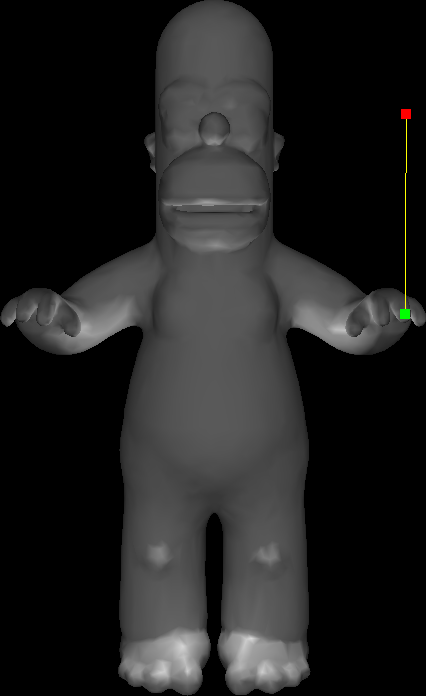
\includegraphics[width=\textwidth]{HomerAnchor.png}
\end{minipage}
\uncover<2->{
\begin{minipage}{0.45\textwidth}
    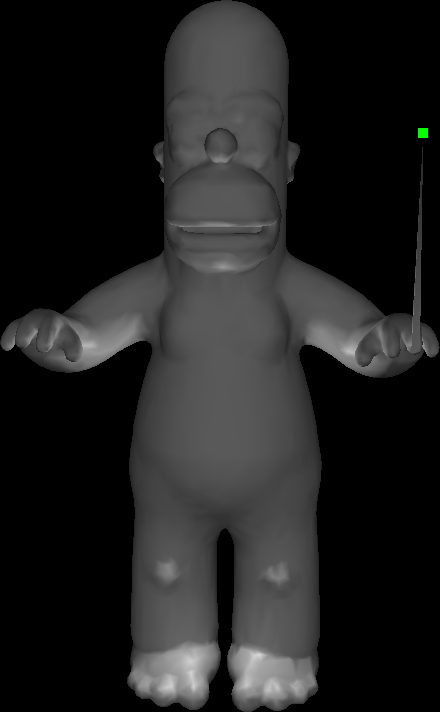
\includegraphics[width=\textwidth]{HomerPointDrag.png}
\end{minipage}
}
\end{figure}

\end{frame}

\begin{frame}{Mesh Editing Overview}

This is not what we want!

\begin{figure}
\begin{minipage}{0.4\textwidth}
    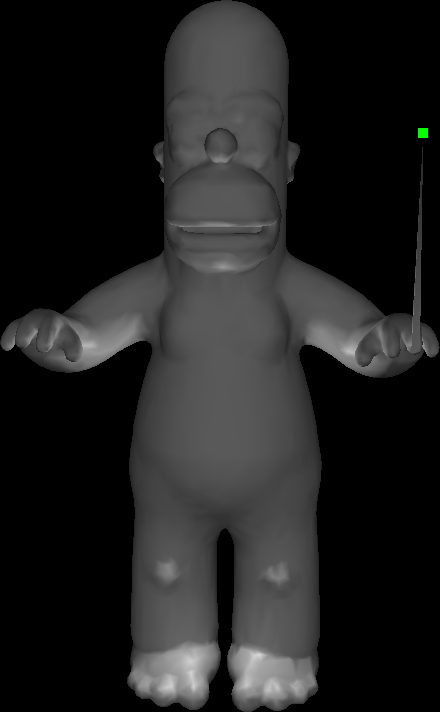
\includegraphics[width=\textwidth]{HomerPointDrag.png}
\end{minipage}
\begin{minipage}{0.4\textwidth}
    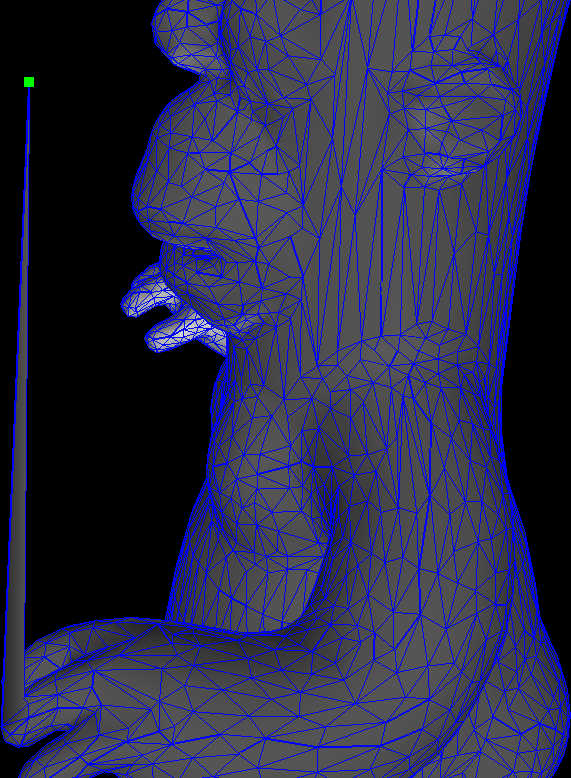
\includegraphics[width=\textwidth]{HomerPointDrag2.png}
\end{minipage}
\end{figure}

\end{frame}


\begin{frame}{Mesh Editing Overview}

\begin{figure}
\begin{minipage}{0.36\textwidth}
    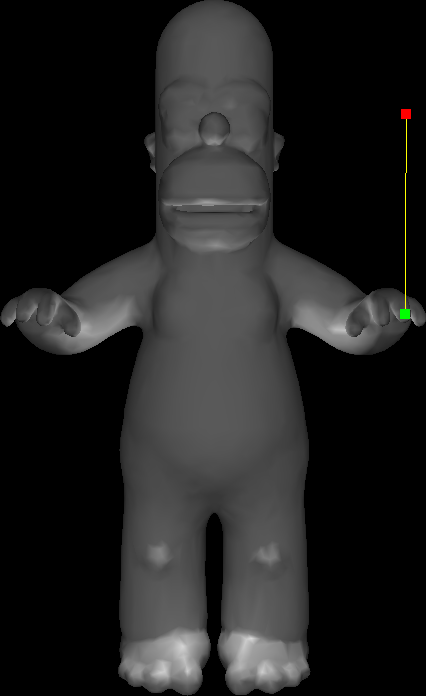
\includegraphics[width=\textwidth]{HomerAnchor.png}
\end{minipage}
\uncover<2->{
\begin{minipage}{0.36\textwidth}
    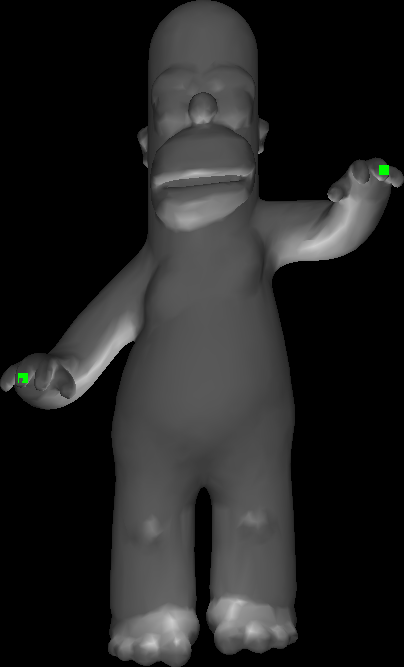
\includegraphics[width=\textwidth]{HomerLaplacian.png}
\end{minipage}
}
\end{figure}

\uncover<2->{
This is much better!  Preserve {\em relative information} about points to neighbors
}

\end{frame}


\begin{frame}{Parameterized Curves / Curvature}

Curvature $\kappa$ is $\frac{1}{r}$, where $r$ is radius of {\em osculating circle}

\begin{figure}[t]
    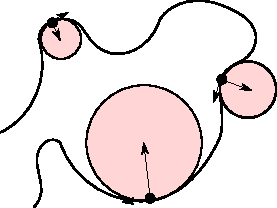
\includegraphics[width=0.6\textwidth]{2DCurvatureVectors.pdf}
\end{figure}

\end{frame}

\begin{frame}{Parameterized Curves / Curvature}

Curvature $\kappa$ is $\frac{1}{r}$, where $r$ is radius of {\em osculating circle}

\begin{figure}[t]
    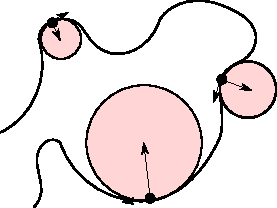
\includegraphics[width=0.5\textwidth]{2DCurvatureVectors.pdf}
\end{figure}

Curvature can also be considered as a vector $\kappa \vec{n}$

\end{frame}

\begin{frame}{Parameterized Curves / Curvature}

\[ \gamma(t) = (x(t), y(t)) \]

Velocity
\[ \gamma'(t) = \left(\frac{d x(t)}{dt}, \frac{d y(t)}{dt} \right) \]

\uncover<2->{
Assume {\em parameterized by arc length}; that is, curve moving at a unit speed.  In other words
\[ \gamma'(t) \cdot \gamma'(t) = 1 \]
}

\uncover<3->{
Differentiate both sides with respect to $t$, use product rule, end up with

\[ 2 \gamma''(t) \cdot \gamma'(t) = 0 \implies \gamma''(t) \perp \gamma'(t) \]

$ \gamma''(t) = \kappa \vec{n(t)} $ is the {\em curvature vector}
}

\end{frame}

%\begin{frame}{Example: Arc Length Parameterized Circles}

%\[ \gamma(t) = \left( \cos(\frac{t}{R} \right) \]

%\end{frame}


\begin{frame}{Discrete Curvature}

\only<1>{
\begin{figure}[t]
    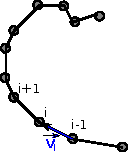
\includegraphics[width=0.3\textwidth]{1DDiscreteDerivative.pdf}
\end{figure}
}

\only<2>{
\begin{figure}[t]
    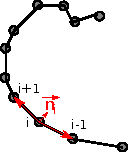
\includegraphics[width=0.3\textwidth]{1DDiscreteCurvature.pdf}
\end{figure}
}

Derivative at point $i$ (velocity vector) is approximately

\[ \textcolor{blue}{\vec{v_i}} = \vec{x_i} - \vec{x_{i-1}} \]

\uncover<2->{

Second derivative (curvature vector) is approximately

\[ \textcolor{red}{\vec{n_i}} = \vec{v_{i+1}} - \vec{v_i} = \vec{x_{i+1}} - \vec{x_{i}} - (\vec{x_{i}} - \vec{x_{i-1}}) = -2\vec{x_i} + \vec{x_{i-1}} + \vec{x_{i+1}} \]



}

\end{frame}

\begin{frame}{Curvature of Surfaces}

Cut surface with plane, look at curvature of curve going through point

\begin{figure}[t]
    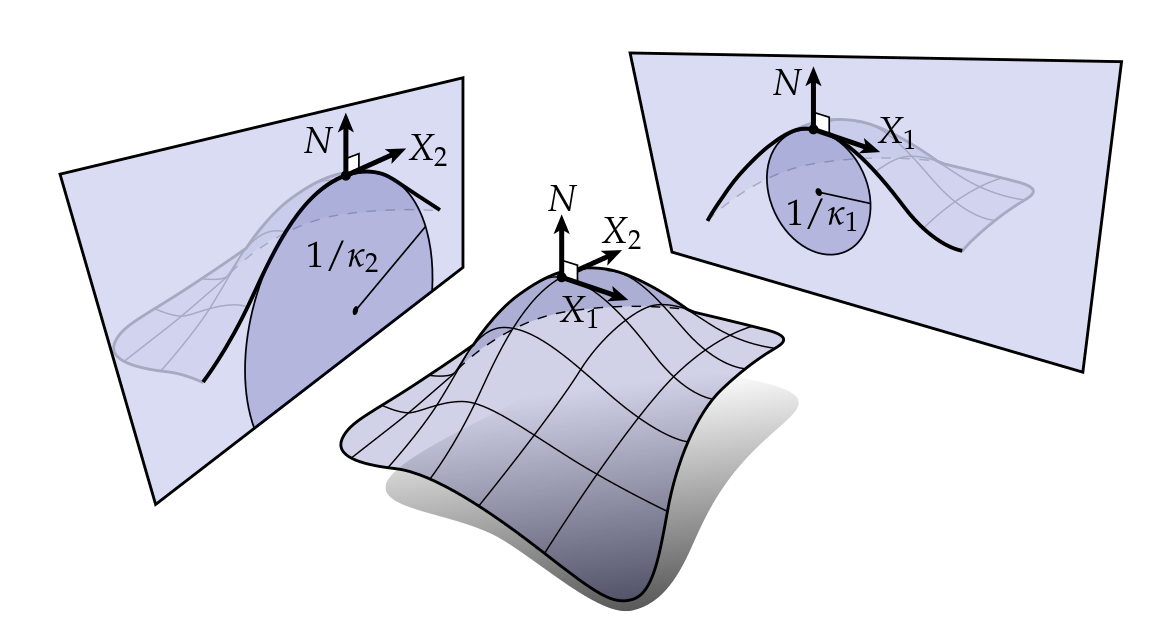
\includegraphics[width=0.8\textwidth]{MeanCurvature.png}
\end{figure}

\small \textcolor{red}{Courtesy of Keenan Crane, {\em Discrete Differential Geometry: An Applied Introduction}}

\end{frame}

\begin{frame}{Discrete Mean Curvature Approximation}

Still just a difference of a point with its neighbors! Convention is \textcolor{red}{negative} the curvature vector: $-H(v_i) \vec{n_i}$, where $H(v_i)$ is the {\em mean curvature}

\begin{itemize}
\item Example with curvature
\begin{figure}[t]
    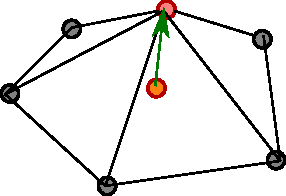
\includegraphics[width=0.36\textwidth]{2DDiscreteCurvature.pdf}
    
\end{figure}

\item Example with flat
\begin{figure}[t]
    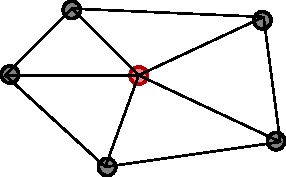
\includegraphics[width=0.36\textwidth]{2DFlat.pdf}
\end{figure}

\end{itemize}

(more details in a moment)

\end{frame}

\begin{frame}{Table of Contents}
\begin{itemize}[label=$\vartriangleright$]
	\item Mesh Editing Overview / Discrete Curvature
\end{itemize}

\begin{itemize}[label=$\blacktriangleright$]
	\item Laplacian Mesh Editing
\end{itemize}
\end{frame}


\begin{frame}{Laplacian Mesh Matrix}

\begin{figure}[t]
    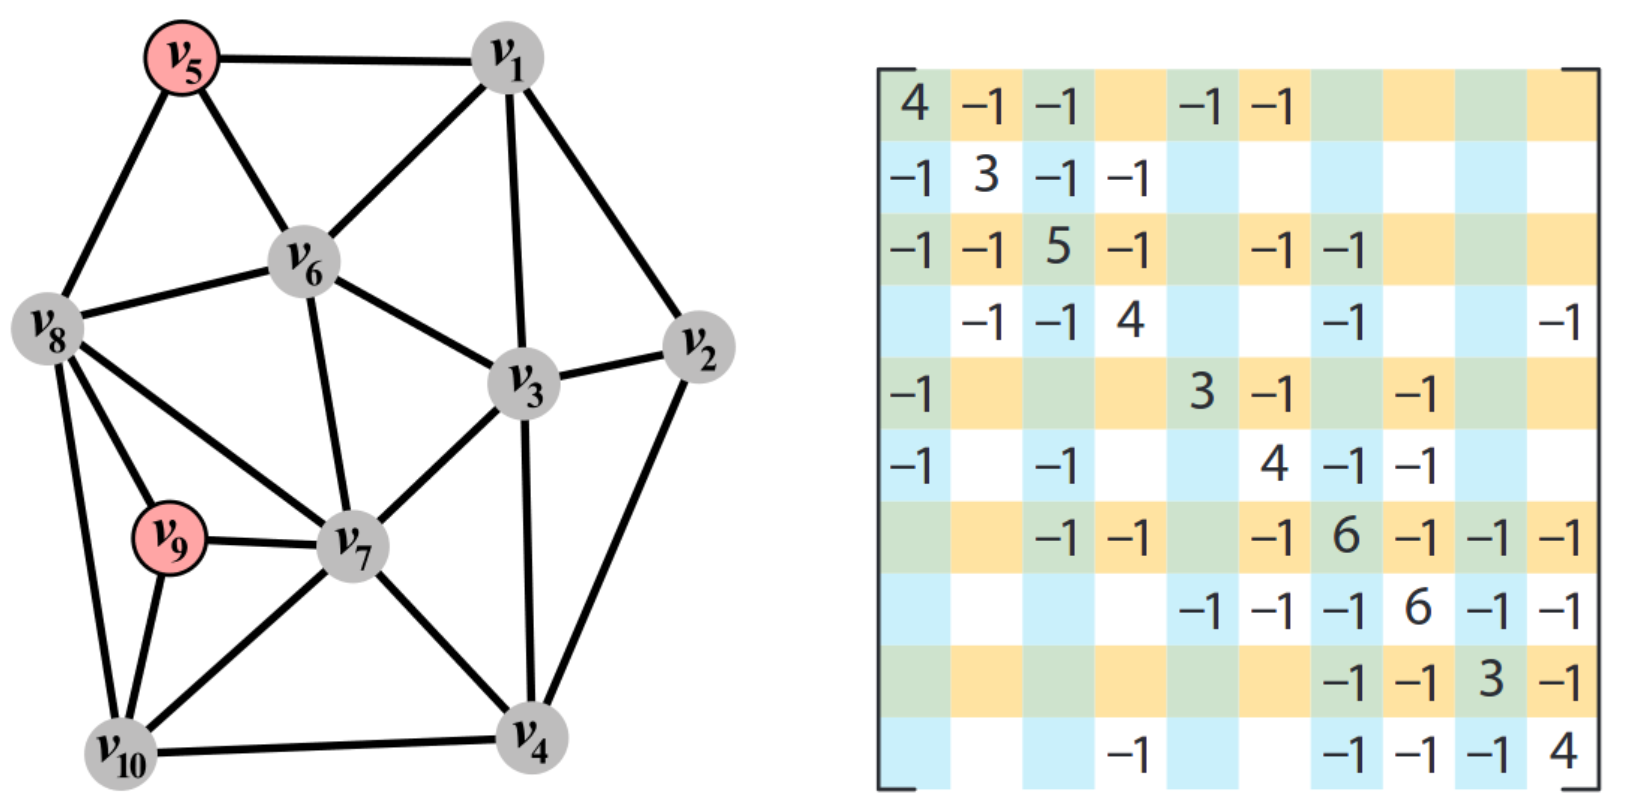
\includegraphics[width=0.8\textwidth]{Sorkine05_GraphLaplacian.png}
\end{figure}

\textcolor{red}{Sorkine05}

\[ L_{ij} = \left\{ \begin{array}{cc} -1 & \text{edge connecting i and j} \\ \text{degree}(i) & i = j \\ 0 & \text{otherwise} \end{array} \right\} \]

\end{frame}


\begin{frame}{Graph Laplacian}

More generally, $L = D - A$

\begin{itemize}[label=$\vartriangleright$]

\item $A$: ``Adjacency matrix''

\[ A_{ij} \left\{ \begin{array}{cc} 1 & \text{edge connecting i and j} \\ 0 & \text{otherwise}  \end{array} \right\} \]

\item $D$: ``Degree matrix''

\[ D_{ij} = \left\{ \begin{array}{cc} \text{degree}(i) = \sum_{j=1}^N A_{ij} & i = j\\ 0 & \text{otherwise} \end{array} \right\} \]

\end{itemize}

L is {\em symmetric} and {\em sparse}.  Number of nonzero entries is $O(N)$ for meshes of constant genus

\end{frame}



\begin{frame}{Laplacian Mesh Editing}

\begin{minipage}{0.45\textwidth}{
\begin{figure}[t]
    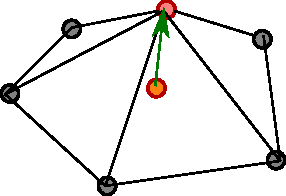
\includegraphics[width=0.7\textwidth]{2DDiscreteCurvature.pdf}
\end{figure}
}
\end{minipage}
\begin{minipage}{0.45\textwidth}
\[ \delta_i = \sum_{j \in N(i)} (v_i - v_j) = d_i v_i - \sum_{j \in N(i)} v_j\]
\end{minipage}


Can be written as $\textcolor{darkgreen}{L} \textcolor{blue}{v} = \textcolor{darkgreen}{\delta}$.  Each vector is {\em along a row} now

\begin{figure}[t]
    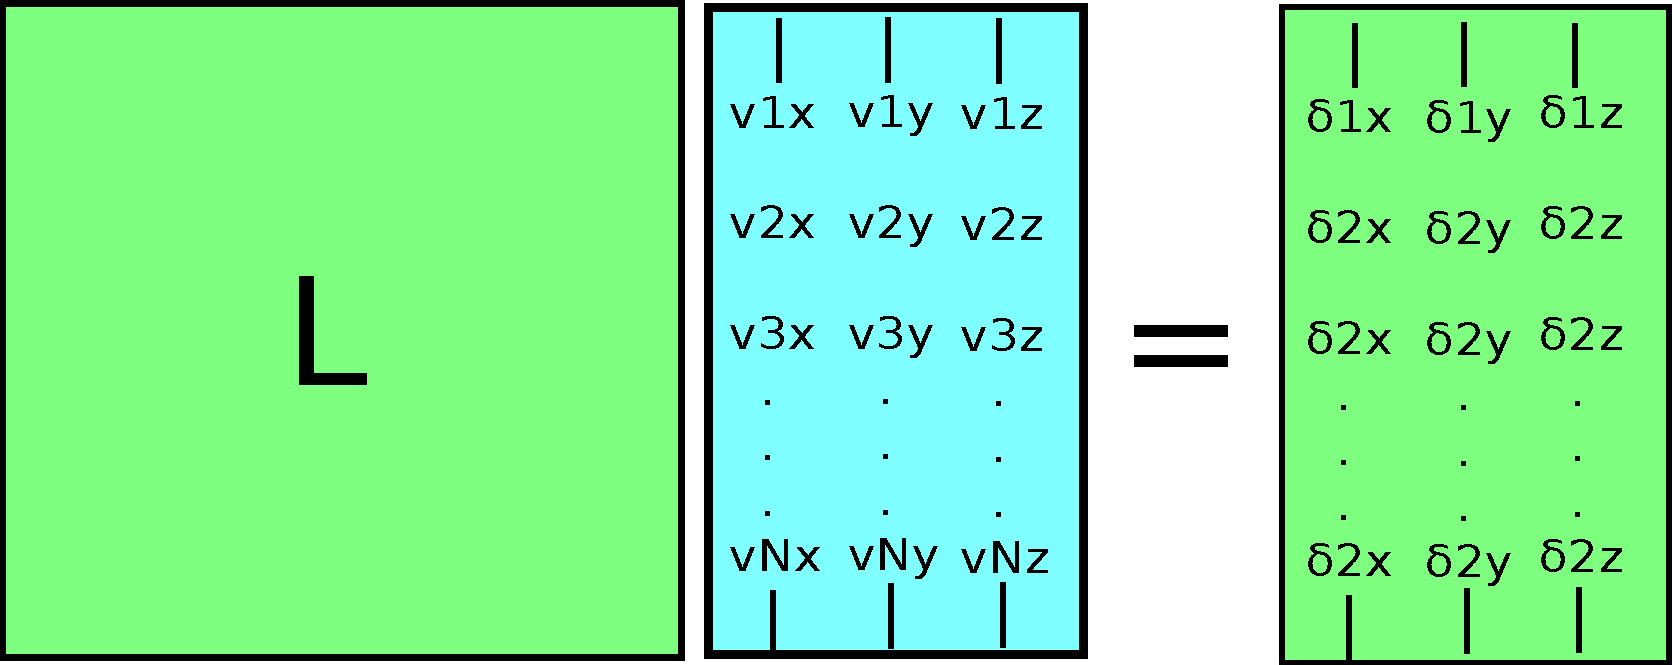
\includegraphics[width=\textwidth]{LaplacianReconstruction.pdf}
\end{figure}


\end{frame}



\begin{frame}{Laplacian Mesh Editing}

\begin{minipage}{0.45\textwidth}{
\begin{figure}[t]
    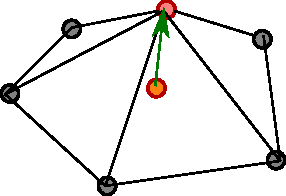
\includegraphics[width=0.7\textwidth]{2DDiscreteCurvature.pdf}
\end{figure}
}
\end{minipage}
\begin{minipage}{0.45\textwidth}
\[ \delta_i = \sum_{j \in N(i)} (v_i - v_j)\]

Can we reconstruct $v$ from $\delta$?
\uncover<2->{
{\em No: $L$ is rank $N-1$ for a connected mesh}
}
\end{minipage}


\begin{figure}[t]
    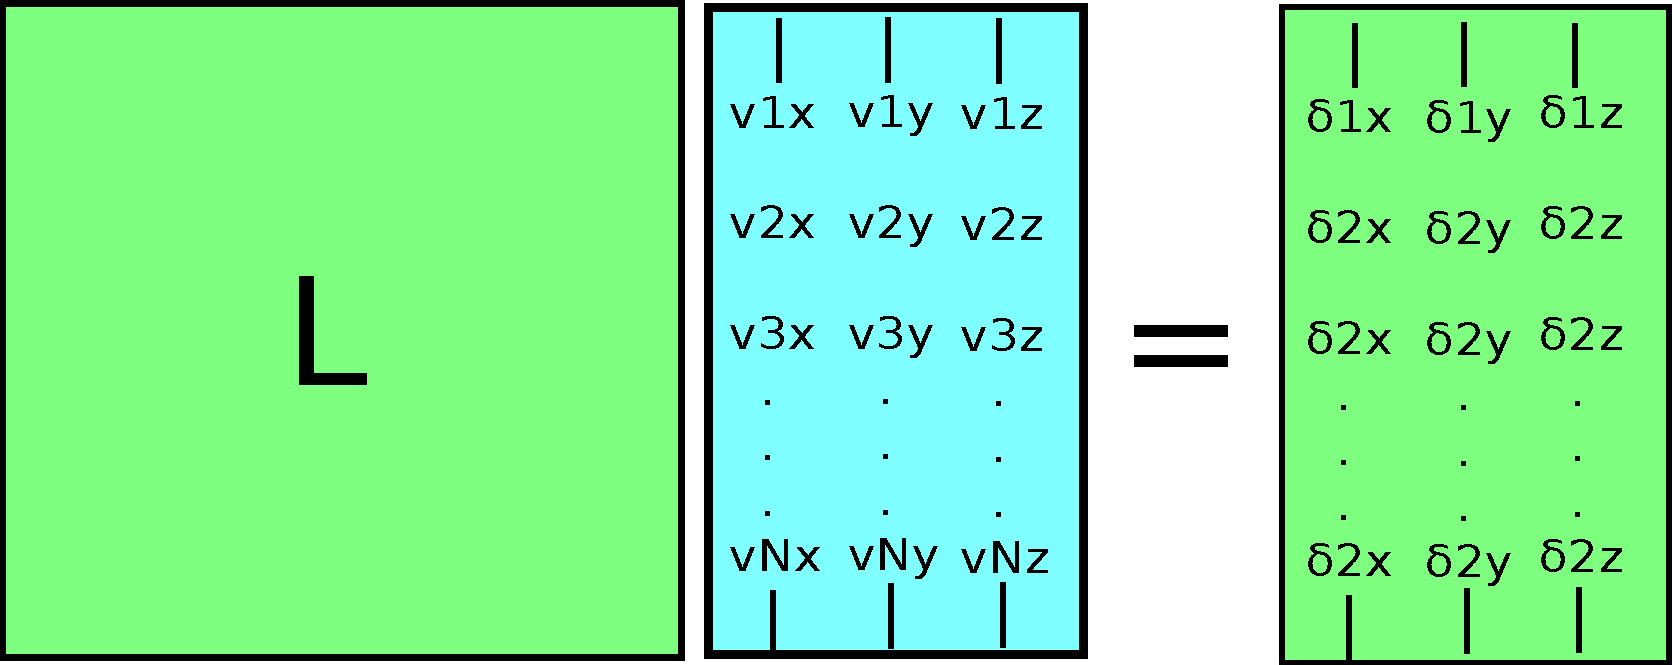
\includegraphics[width=\textwidth]{LaplacianReconstruction.pdf}
\end{figure}


\end{frame}


\begin{frame}{Laplacian Mesh Editing: Anchors}

\begin{minipage}{0.45\textwidth}{
\begin{figure}[t]
    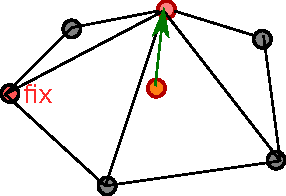
\includegraphics[width=0.7\textwidth]{2DDiscreteCurvatureAnchor1.pdf}
\end{figure}
}
\end{minipage}
\begin{minipage}{0.45\textwidth}
\[ \delta_i = \sum_{j \in N(i)} (v_i - v_j)\]

Delta coordinates define geometry {\em up to a translation}.  Fix a point $v_a$, fix translation
\end{minipage}

\begin{figure}[t]
    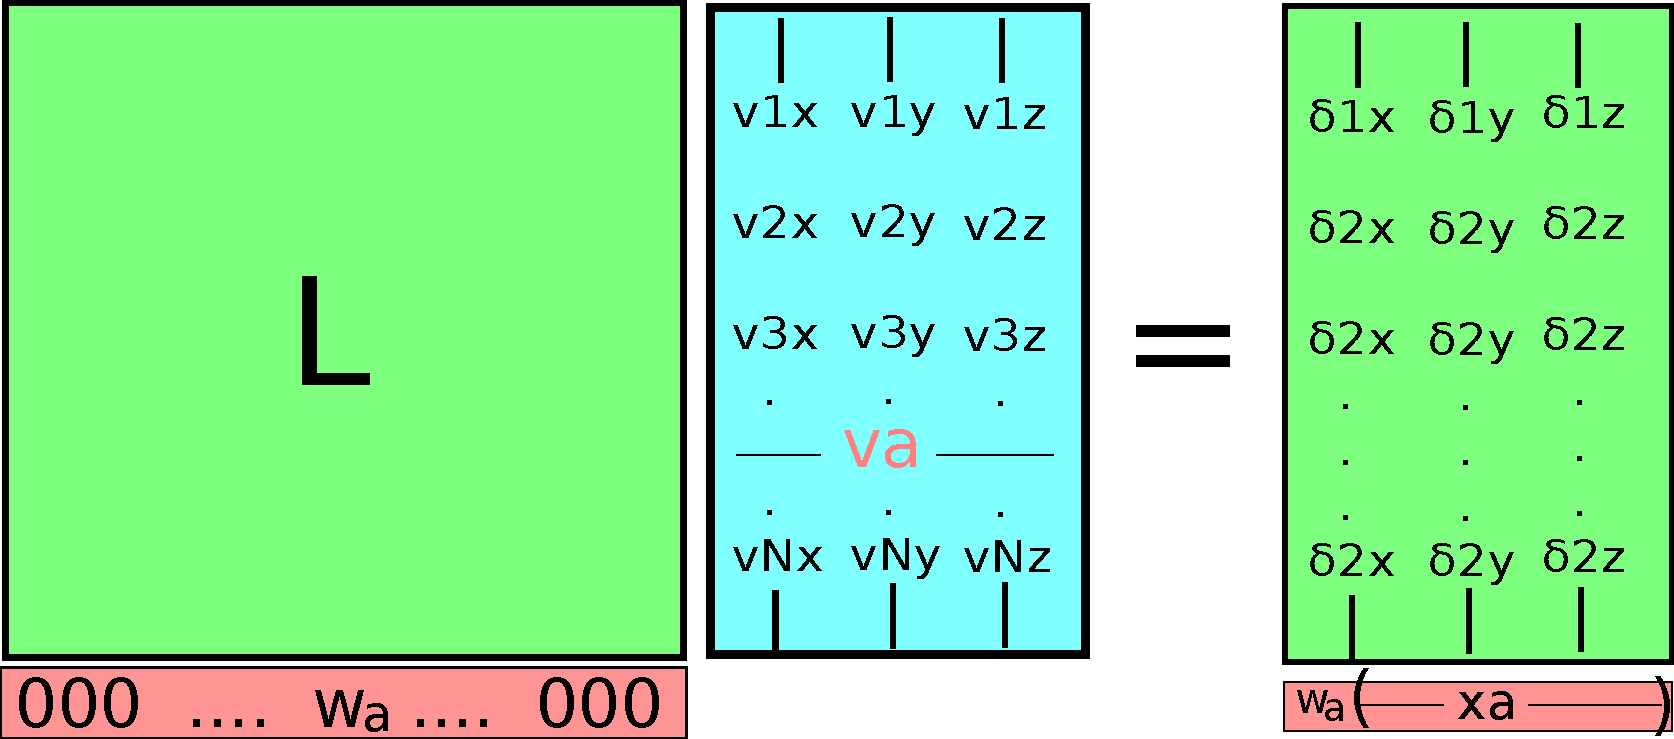
\includegraphics[width=0.8\textwidth]{LaplacianReconstruction1Anchor.pdf}
\end{figure}

\end{frame}


\begin{frame}{Laplacian Mesh Editing: Anchors}

\begin{minipage}{0.45\textwidth}{
\begin{figure}[t]
    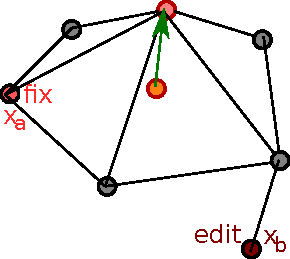
\includegraphics[width=0.7\textwidth]{2DDiscreteCurvatureAnchor2.pdf}
\end{figure}
}
\end{minipage}
\begin{minipage}{0.45\textwidth}
Can add more anchors, but may not be a solution
\uncover<2->{
Solve in the {\em least squares sense}
\[ \widetilde{v} = \text{argmin}_v ||\textcolor{green}{L}\textcolor{blue}{v} - \textcolor{green}{\delta} ||_2^2 + \sum_{s = 1}^k w_s ||\textcolor{blue}{v_s} - \textcolor{red}{x_s}||_2^2 \]
}
\end{minipage}

\begin{figure}[t]
    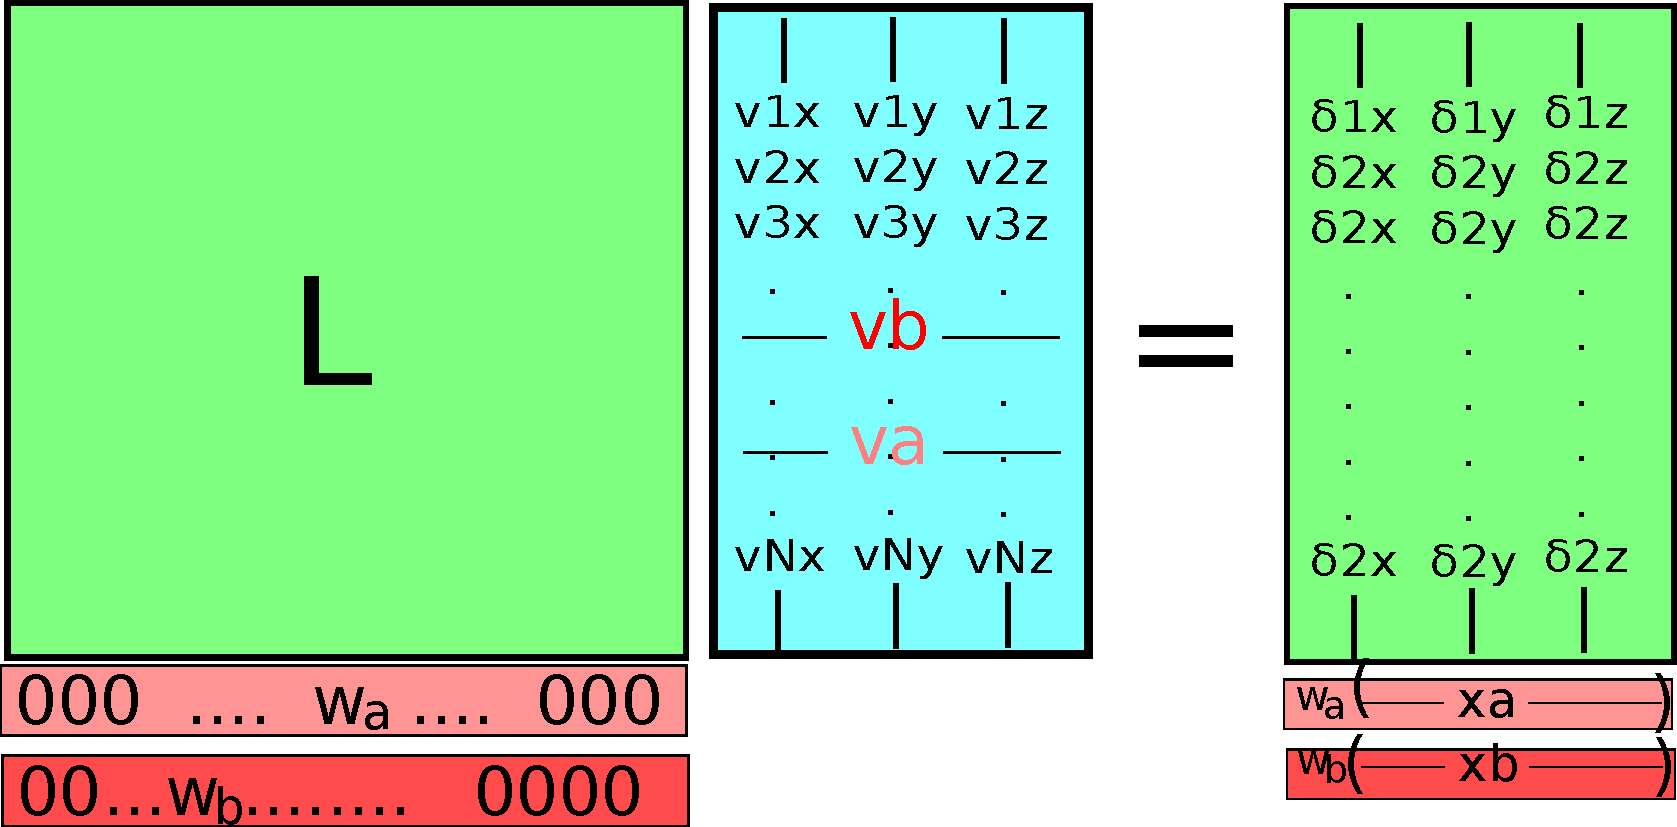
\includegraphics[width=0.8\textwidth]{LaplacianReconstruction2Anchor.pdf}
\end{figure}

\end{frame}

\begin{frame}{Laplacian Mesh Editing: Anchors: Another Example}


\end{frame}

\begin{frame}{Laplacian Mesh Editing: Anchors}


\[ \widetilde{v} = \text{argmin}_v ||\textcolor{green}{L}\textcolor{blue}{x} - \textcolor{green}{\delta} ||_2^2 + \sum_{s = 1}^k w_s ||\textcolor{blue}{x_s} - \textcolor{red}{v_s}||_2^2 \]

\uncover<2->{
\begin{itemize}[label=$\vartriangleright$]
\item Let $\overline{L}$ be $L$ augmented with the anchor rows
\item Let $\overline{\delta}$ be $\delta$ augmented with the weighted anchor coordinates
\end{itemize}

Can all be written in matrix form

\[ \text{Squared Error: } \epsilon(v) = ||\overline{L}v - \overline{\delta} ||_2^2 \]

\[ \text{Least Squares Solution: } v^* = (\overline{L}^T \overline{L})^{-1} \overline{L}^T \overline{\delta} \]

}

\end{frame}

\begin{frame}{Laplacian Mesh Editing: Examples}

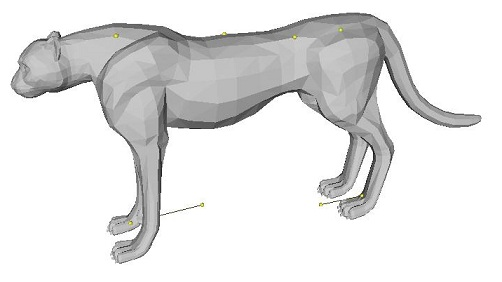
\includegraphics[width=0.6\textwidth]{deform1_1.jpg}

\uncover<2->{
\begin{figure}[t]
    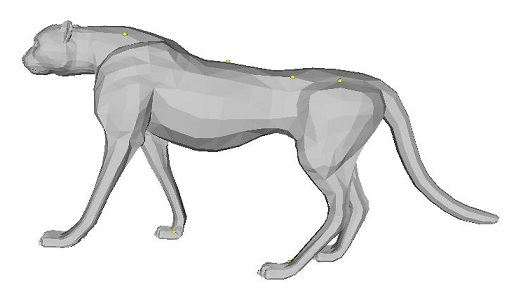
\includegraphics[width=0.6\textwidth]{deform1_2.jpg}
\end{figure}
}

\end{frame}


\begin{frame}{Laplacian Mesh Editing: Examples}



\begin{figure}
\begin{minipage}{0.45\textwidth}
    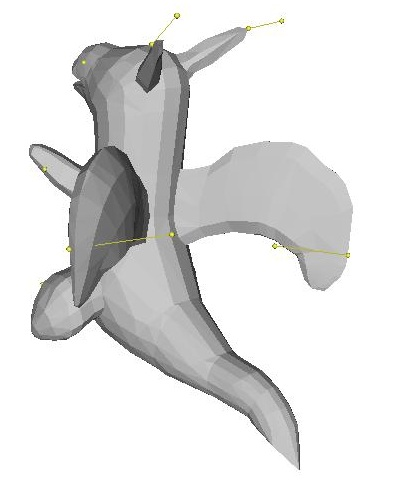
\includegraphics[width=\textwidth]{deform5_1.jpg}
\end{minipage}
\uncover<2->{
\begin{minipage}{0.5\textwidth}
    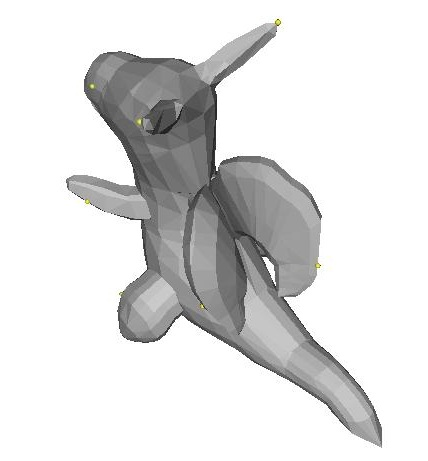
\includegraphics[width=\textwidth]{deform5_2.jpg}
\end{minipage}
}
\end{figure}



\end{frame}

\begin{frame}{What About Irregular Meshes?}

\begin{figure}[t]
    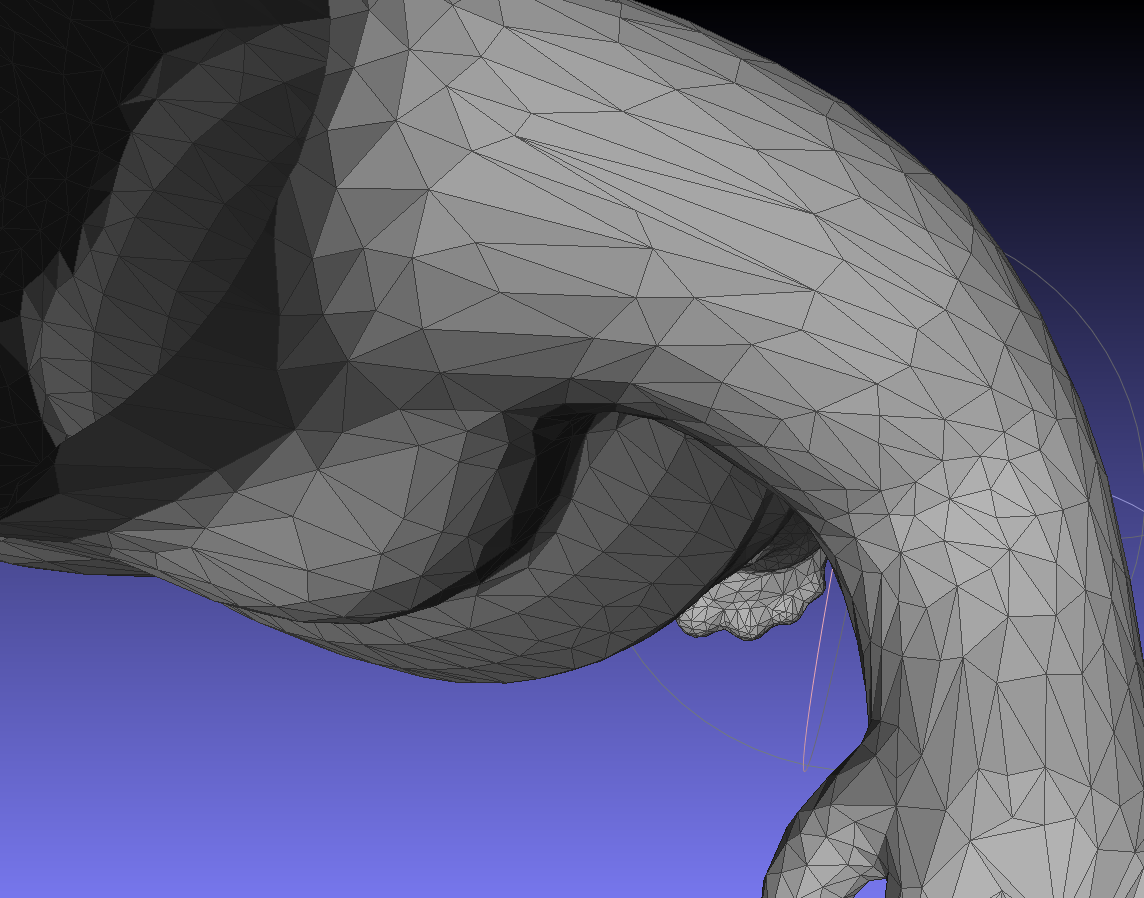
\includegraphics[width=0.8\textwidth]{HomerIrregular.png}
\end{figure}

Homer's upper arm

\end{frame}

\begin{frame}{Cotangent Weights}

\begin{figure}
\begin{minipage}{0.45\textwidth}
    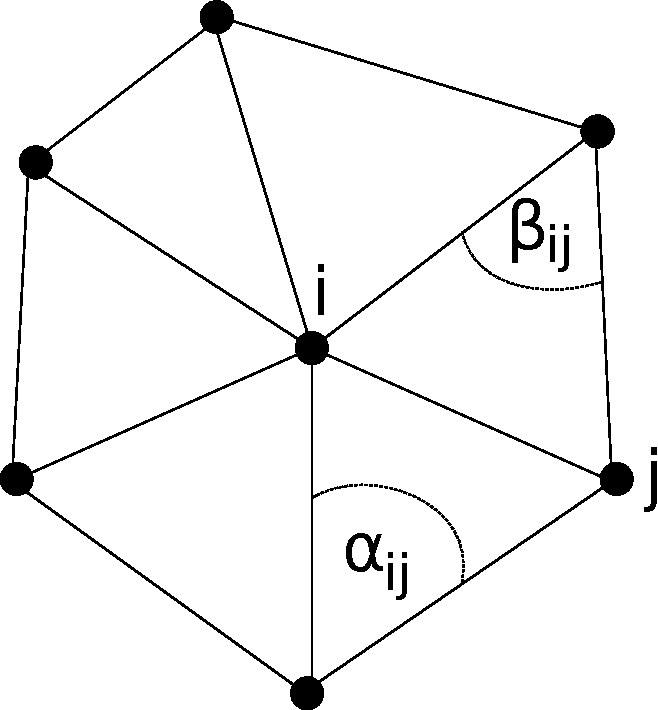
\includegraphics[width=0.8\textwidth]{DiscretizedLaplacian.pdf}
    \[ \delta_i = \sum_{j \in N(i)} w_{ij}(v_i - v_j) \]
    \[ w_{ij} = \frac{1}{2}( \cot(\beta_{ij}) + \cot(\alpha_{ij}))\]
\end{minipage}
\uncover<2->{
\begin{minipage}{0.5\textwidth}
    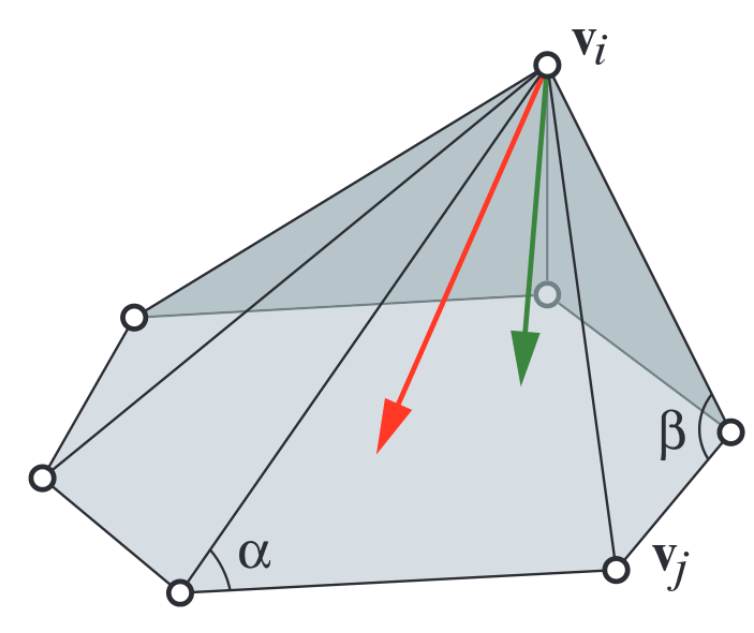
\includegraphics[width=\textwidth]{Nealen2006.png}
    \caption{Nealen2006, \textcolor{red}{umbrella} vs \textcolor{darkgreen}{cotangent}}
\end{minipage}
}
\end{figure}


\end{frame}

\begin{frame}{Cotangent Weights: Mean Curvature}


Mean curvature is approximated by

\[ \frac{1}{2} \sum_{j \in N(i)}  (\cot(\beta_{ij}) + \cot(\alpha_{ij}))||\vec{v_i} - \vec{v_j}||_2 \]

\begin{figure}[t]
    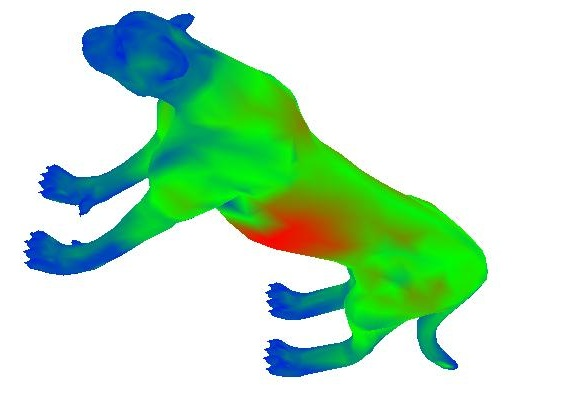
\includegraphics[width=0.7\textwidth]{curv2_1.jpg}
\end{figure}

\end{frame}

\begin{frame}{Laplacian Mesh Editing: Umbrella vs Cotangent}

\begin{figure}
\begin{minipage}{0.45\textwidth}
    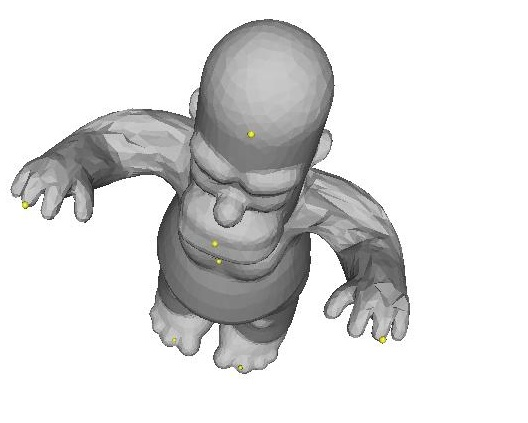
\includegraphics[width=\textwidth]{homer_umbrella.jpg}
    \caption{\textcolor{red}{umbrella}}
\end{minipage}
\uncover<2->{
\begin{minipage}{0.5\textwidth}
    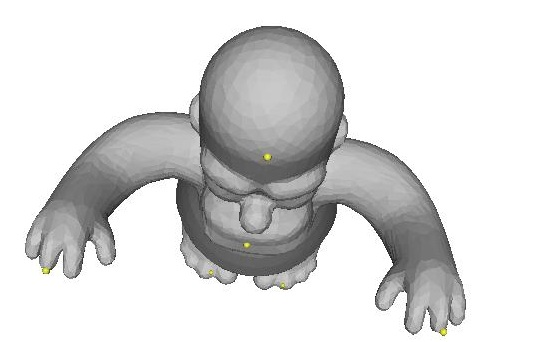
\includegraphics[width=\textwidth]{homer_cotangent.jpg}
    \caption{\textcolor{darkgreen}{cotangent}}
\end{minipage}
}
\end{figure}

\end{frame}


\begin{frame}{Laplacian Mesh Editing: Umbrella vs Cotangent}

\begin{figure}
\begin{minipage}{0.45\textwidth}
    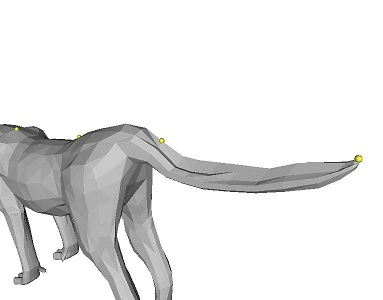
\includegraphics[width=\textwidth]{cheetahtail_umbrella.jpg}
    \caption{\textcolor{red}{umbrella}}
\end{minipage}
\uncover<2->{
\begin{minipage}{0.5\textwidth}
    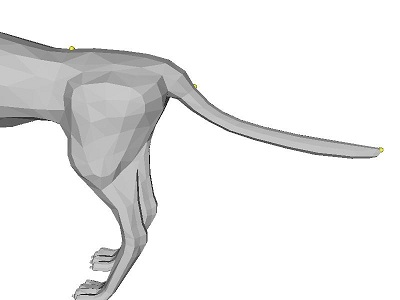
\includegraphics[width=\textwidth]{cheetahtail_cotangent.jpg}
    \caption{\textcolor{darkgreen}{cotangent}}
\end{minipage}
}
\end{figure}

\end{frame}

\begin{frame}{Applications: Function Interpolation}

\begin{figure}[t]
    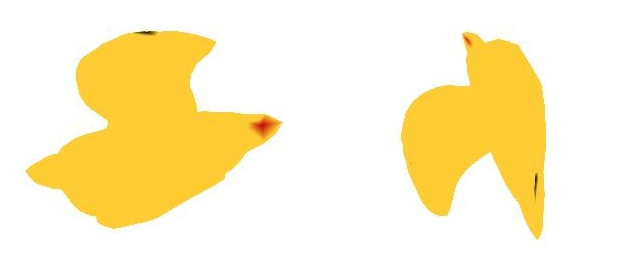
\includegraphics[width=0.7\textwidth]{FunctionSpecification.png}
\end{figure}

\uncover<2->{
\begin{figure}[t]
    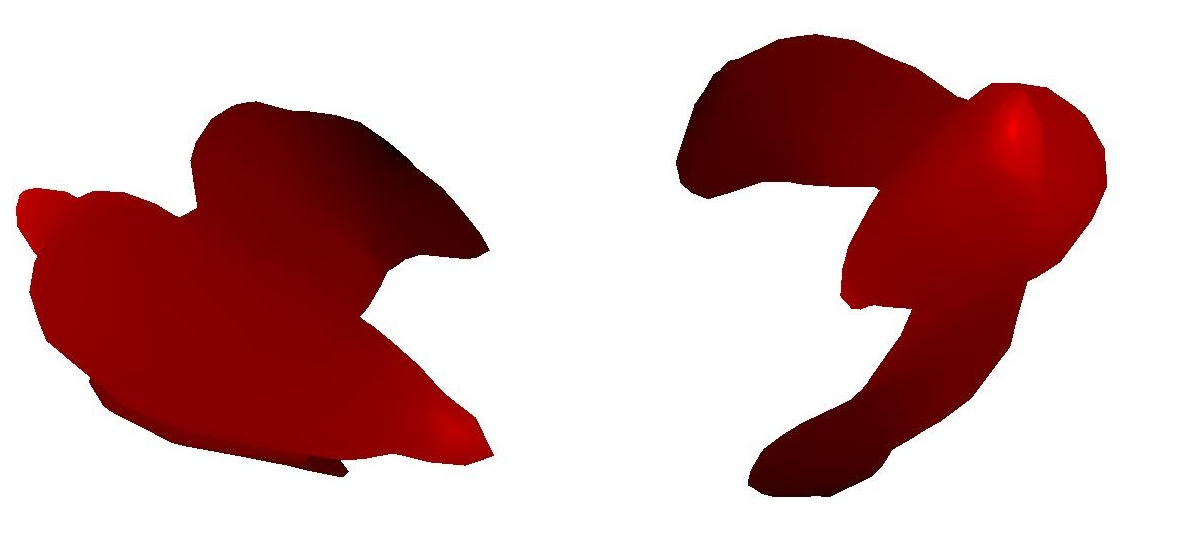
\includegraphics[width=0.7\textwidth]{FunctionInterpolation.png}
\end{figure}
}

\end{frame}

\begin{frame}{Applications: Detail Transfer / Mesh Mixing}

\begin{figure}[t]
    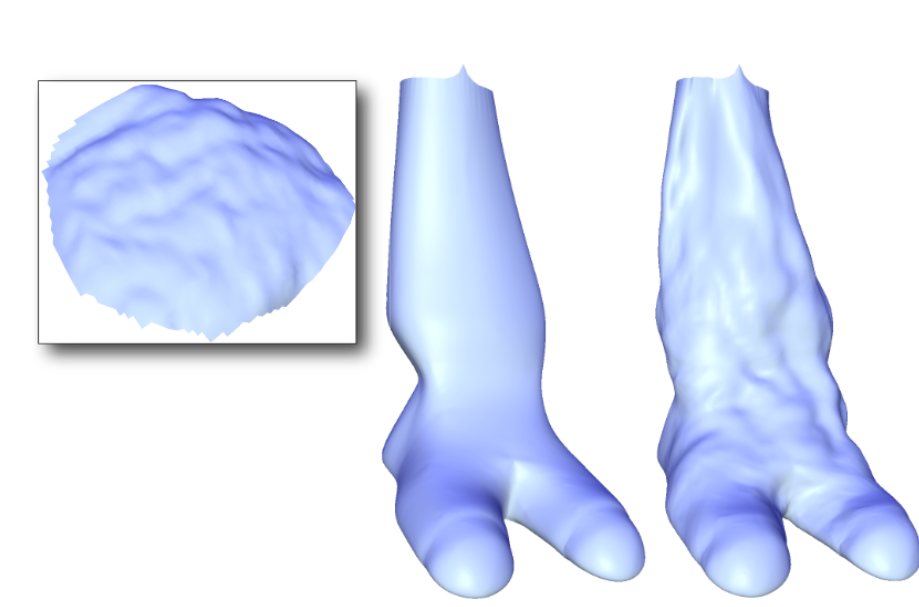
\includegraphics[width=\textwidth]{Sorkine05_ShapeBlending2.png}
\end{figure}

\textcolor{red}{Sorkine 05}

\end{frame}

\begin{frame}{Applications: Detail Transfer / Mesh Mixing}

\begin{figure}[t]
    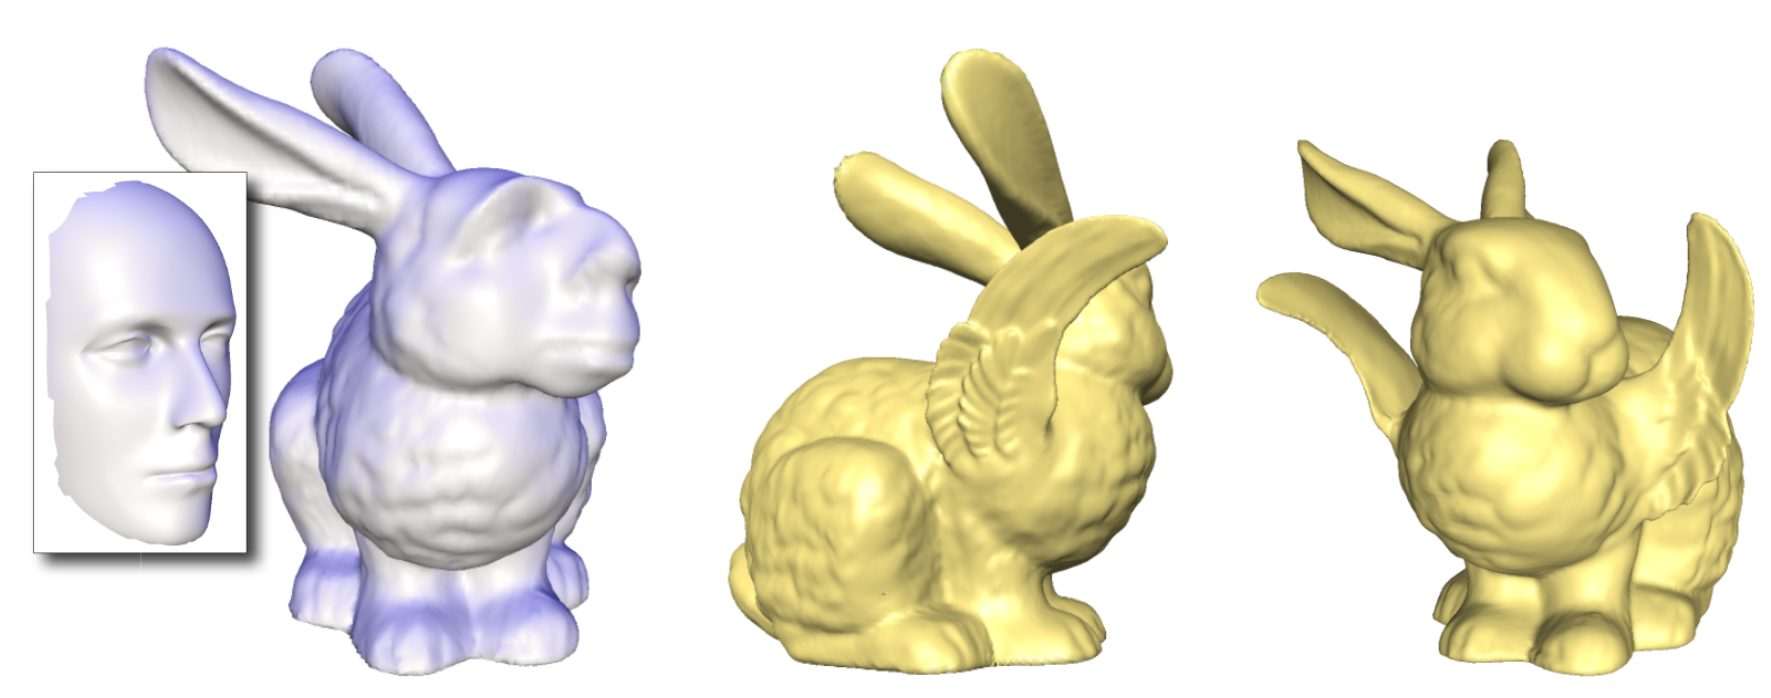
\includegraphics[width=\textwidth]{Sorkine05_ShapeBlending1.png}
\end{figure}

\textcolor{red}{Sorkine 05}

\end{frame}

\begin{frame}{Applications}

More surprises in group assignment 3 and the following lectures!

\end{frame}

\begin{frame}{A Note About Rotation Invariance}

\[ \textcolor{darkgreen}{L} \textcolor{blue}{x} = \textcolor{darkgreen}{\delta} \]

\begin{itemize}[label=$\vartriangleright$]
\item $\delta$ is a {\em vector}.  $||\delta|| \propto \kappa$, but it has a direction
\end{itemize}

\begin{figure}[t]
    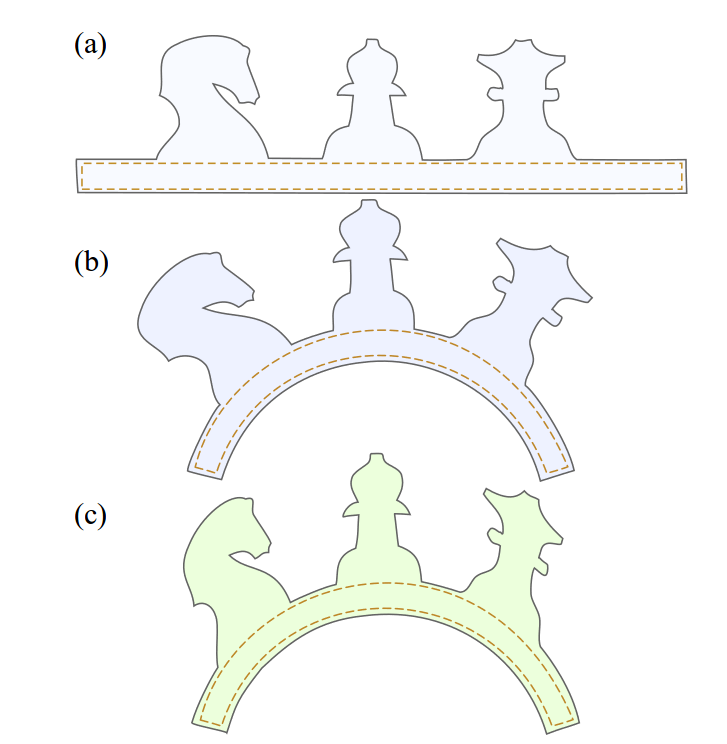
\includegraphics[width=0.5\textwidth]{Sorkine05.png}
    \caption{\textcolor{red}{Sorkine05}}
\end{figure}

\end{frame}

\begin{frame}{As Rigid As Possible Surface Editing}

\begin{figure}[t]
    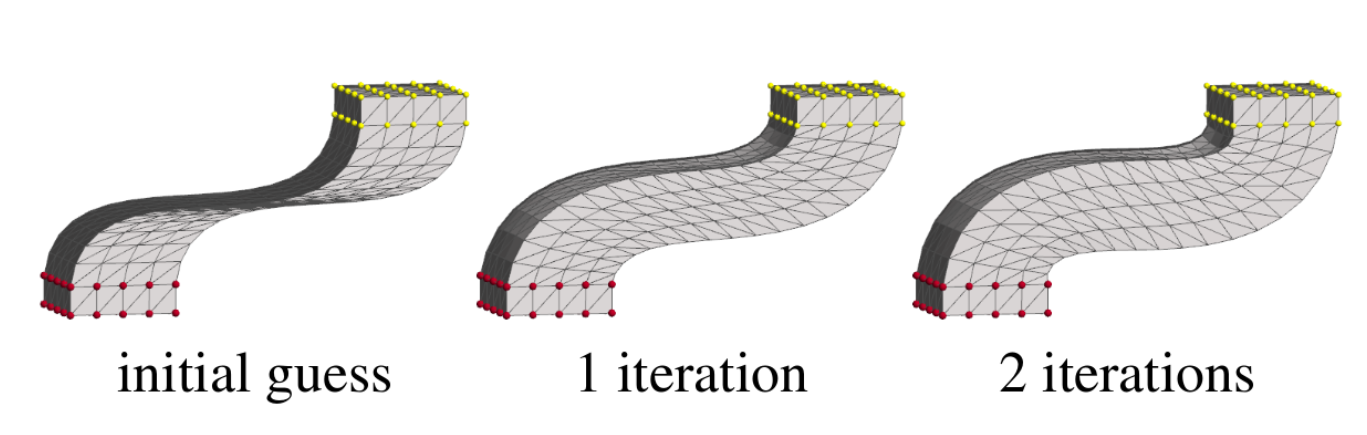
\includegraphics[width=\textwidth]{Sorkine07_1.png}
\end{figure}

\uncover<2->{
\begin{figure}[t]
    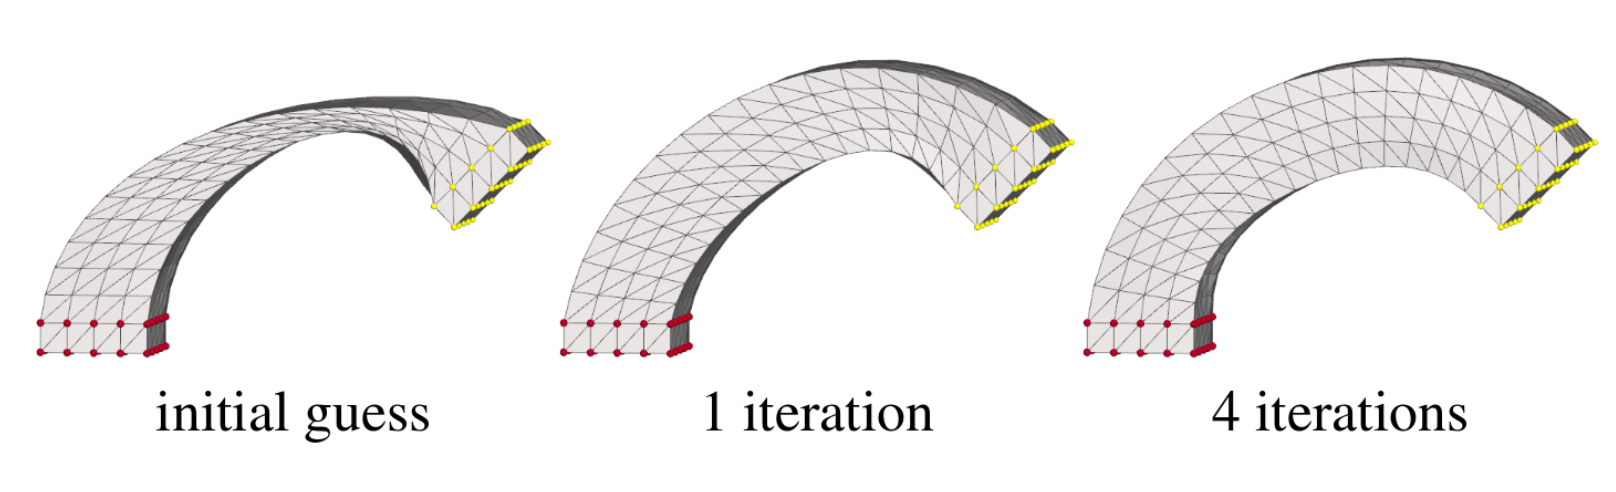
\includegraphics[width=\textwidth]{Sorkine07_2.png}
\end{figure}
}

\textcolor{red}{Sorkine2007}

\end{frame}


\begin{frame}{A Note On Sparse Matrices}

Sparse matrices in numpy

\end{frame}


\end{document}

